\documentclass[pdflatex,a4paper,11pt,titlepage]{article}

%% Load packages ========================================
\usepackage[T1]{fontenc}

%\usepackage{xr-hyper} % needs to be loaded before hyperref
\usepackage{ifpdf,ifxetex}
\ifxetex
  \usepackage{epstopdf}
  \epstopdfsetup{suffix=.\SourceExt}
  \usepackage{fontspec}           % XeLaTeX specific
  \defaultfontfeatures{Mapping=tex-text} % For archaic input (e.g. convert -- to en-dash)
  \setmainfont{Linux Libertine O}  % LaTeX default (Computer Modern Unicode)
  \usepackage[xetex,colorlinks,unicode=True]{hyperref}
\else
  \usepackage[utf8]{inputenc}     % support utf8 (if possible: use xetex)
  \usepackage{lmodern}
  \usepackage{newunicodechar}
  \ifpdf
    \usepackage[pdftex]{graphicx}
    \usepackage{epstopdf}
    \epstopdfsetup{suffix=.\SourceExt}
    \usepackage[pdftex,colorlinks,unicode=True]{hyperref}
  \else
    \usepackage{graphicx}
    \usepackage[colorlinks,unicode=True]{hyperref}
  \fi
\fi
\usepackage[dvipsnames]{xcolor}
\usepackage{subfig}

\usepackage{booktabs} % <--- This is the way to do it if you ask me.

\usepackage[absolute,overlay]{textpos} % textblock (see inc/kth_titlepage)

\usepackage{authblk}
\renewcommand\Authsep{, }
\renewcommand\Authand{ och }
\renewcommand\Authands{, och }
%\renewcommand*{\thefootnote}{\fnsymbol{footnote}}
\usepackage[perpage]{footmisc} % \cite => numbers
\renewcommand{\thefootnote}{\fnsymbol{footnote}}
\usepackage[style=chem-acs,doi,autocite=superscript,pageranges=false,backend=biber]{biblatex}
\AtEveryBibitem{\clearfield{month}} % Don't put "Jan. 2000" in references
\AtEveryCitekey{\clearfield{month}} % http://tex.stackexchange.com/questions/55780
\renewcommand{\cite}{\autocite}
\usepackage{amsmath, amsfonts, amssymb, amsthm}
\usepackage{siunitx}
\DeclareSIUnit\molar{\mole\per\cubic\deci\metre}
\DeclareSIUnit\Molar{\textsc{m}}
\usepackage[version=3]{mhchem}
%\usepackage{chemstyle}  % \standardstate symbol
\newcommand*{\plimsoll}{{\ensuremath{-\kern-5pt{\circ}\kern-5pt-}}} % standard state symbol

% Make References appear in Table of Contents
\usepackage[nottoc,notlof,notlot,numbib]{tocbibind}

\hypersetup{%
  bookmarksnumbered=true, %
  breaklinks=false, %
  raiselinks=true, %
  pdfborder={0 0 0}, %
  colorlinks=true, %
  plainpages=false, %
  pdfstartview={FitH}, %
  pdfcreator={LaTeX with hyperref package}, %
  citecolor=teal, % See xcolor package documentation
  linkcolor=Maroon, %
  urlcolor=blue, %
}%

\usepackage{minted}

% Minted matlab code
\definecolor{mintedbackground}{rgb}{0.95,0.95,0.95}

\newmintedfile[matlabcode]{matlab}{
bgcolor=mintedbackground,
fontfamily=tt,
fontsize=\footnotesize,
linenos=true,
numberblanklines=true,
numbersep=12pt,
numbersep=5pt,
gobble=0,
frame=leftline,
framerule=0.4pt,
framesep=2mm,
funcnamehighlighting=true,
tabsize=4,
obeytabs=false,
mathescape=false
samepage=false, %with this setting you can force the list to appear on the same page
showspaces=false,
showtabs =false,
texcl=false,
}
%% Global Last Commands
\usepackage[capitalise,noabbrev,swedish]{cleveref} % <--- Needs to be loaded late (see doc)
\usepackage{listings}

\lstnewenvironment{terminaloutput}{%
  \lstset{backgroundcolor=\color{mintedbackground},
  frame=single,
  breaklines=true,
  framerule=0pt,
  basicstyle=\footnotesize\ttfamily,
  columns=fullflexible}}{}

\renewcommand{\thesection}{C\arabic{section}} % Bilaga

\providecommand{\projecttitle}{Övningsuppgift -- Stopped flow \\ KD1080}
\hypersetup{%
  pdfkeywords={stopped flow},%
  pdfauthor={Björn Dahlgren},%
  pdftitle={KD1080 \projecttitle}%
}
\providecommand{\mailto}{\texttt{\href{mailto:bda@kth.se}{bda@kth.se}}}
\author[1]{Björn Dahlgren (\mailto)}
\affil[1]{School of Chemical Science and Engineering, Applied Physical Chemistry, KTH}

\title{\projecttitle}


\begin{document}
 
  %% Non-fancy:  ---------------------------------------------------
% \begin{titlepage}
%   \maketitle
% \end{titlepage}

%% Fancy:      ---------------------------------------------------

\makeatletter
    \begin{titlepage}
\begin{textblock*}{2cm}(12mm,12mm) % {block width} (coords)

\includegraphics[width=2cm]{fig/kth.pdf}
\end{textblock*}
      % \begin{picture}(1,1)
      %   \put(0,0){\hbox{
\includegraphics[width=2cm]{fig/kth.pdf}}}
      % \end{picture}
      \begin{center}
        ~\\[20ex]
            {\LARGE \bfseries \sffamily \@title }\\[4ex]
            {\Large  \@author}\\[4ex]
            \@date \\[14ex]
            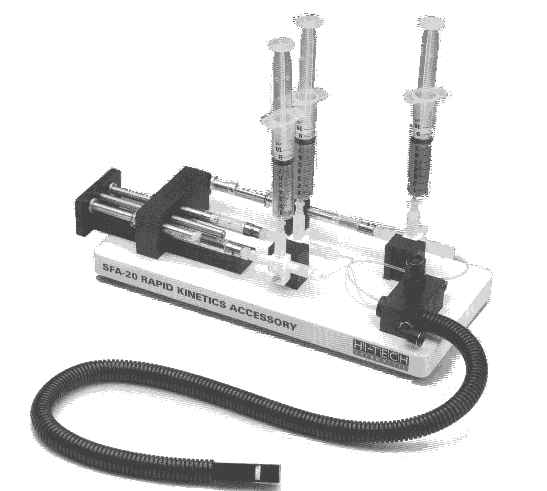
\includegraphics[width=4cm]{fig/setup_bw3.jpg}
        \end{center}
    \end{titlepage}
\makeatother
\thispagestyle{empty}
\newpage

%Add content for page two here (useful for two-sided printing)
\thispagestyle{empty}
\newpage

\setcounter{page}{1} %Start the actually document on page 1


  % \tableofcontents
  % \listoffigures
  %\listoftables
  % \pagebreak

  \setlength{\parindent}{0em}
  \setlength{\parskip}{1em}


  \section{Övningsuppgift för dataanalys}
\label{sec:exercise}
Antag att ni upptäckt följande exotiska reaktion:

\begin{align}
  \label{eq:fourth-order}
  \ce{3A + B ->[k_f] C}
\end{align}

Reaktionen antas vara av tredje ordningen med avseende på A och första
ordningen med avseende på B. Ämne A är starkt färgat medan B och C är
färglösa.

Ni genomför ett antal experiment där ni varierar initialhalten av B enligt
följande: \SI{0.1}{\Molar}, \SI{0.2}{\Molar}, \SI{0.3}{\Molar}, \SI{0.4}{\Molar},
\SI{0.5}{\Molar}. Startkoncentrationen av A är alltid
\SI{1}{\milli\Molar}. Ni använder en \SI{1}{\cm} kyvett i ett
termostaterat rum (\SI{298.15}{\kelvin}), ni mäter vid
$\lambda_{max}=\SI{653}{\nano\metre}$.

För varje halt av B upprepar ni försöket 10 gånger. Under varje försök
antecknar ni vid 42 olika tidpunkter värden för absorbansen på lösningen.
Ni märker att ett par av era serier innehåller väldigt höga brusnivåer
(ni misstänker någon form av elektrisk störning).

Er uppgift är nu att bestämma hastighetskonstanten $k_f$. Mätdata för
analysen hittar ni i filen {\tt data.zip}. Filen innehåller fem mappar
(mappnamn är [B]$_0$ i molar) med vardera tio filer (replikat). Filerna
innehåller två kolumner: tid (i sekunder) och absorbans (enhetslös).

Notera att ni skall använda samtliga datafiler i analysen och ni skall
inte välja ut data för hand, utan istället skall ni använda er av
statistisk analys (viktad regression).

Tips: se om ni kan göra någon förenkling med tanke på initialhalter.

%%% Local Variables:
%%% mode: latex
%%% TeX-master: "../exercise"
%%% ispell-local-dictionary: "swedish"
%%% End:


\end{document}
